\chapter*{Phụ lục A. Luật rút trích thông tin bài báo khoa học}
\addcontentsline{toc}{chapter}{Phụ lục A. Xây dựng và làm giàu kho dữ liệu học thuật}
\ifpdf
    \graphicspath{{Appendix1/Appendix1Figs/PNG/}{Appendix1/Appendix1Figs/PDF/}{Appendix1/Appendix1Figs/}}
\else
    \graphicspath{{Appendix1/Appendix1Figs/EPS/}{Appendix1/Appendix1Figs/}}
\fi

%Phần này sẽ trình bày giải pháp cho rút trích, xây dựng kho dữ liệu khoa học bằng cách tích hợp từ nhiều nguồn không đồng nhất (hình \ref{fig:figure_A_1}). Bên cạnh việc thu thập và làm giàu kho dữ liệu khoa học, luận án cũng xem xét giải quyết vấn đề nhập nhằng tên tác giả trong kho dữ liệu và cuối cùng là các mạng xã hội học thuật sẽ được rút trích, mô hình từ kho dữ liệu khoa học này.
%\begin{figure}[ht]
%\begin{center}
%\advance\leftskip-3cm
%\advance\rightskip-3cm
%  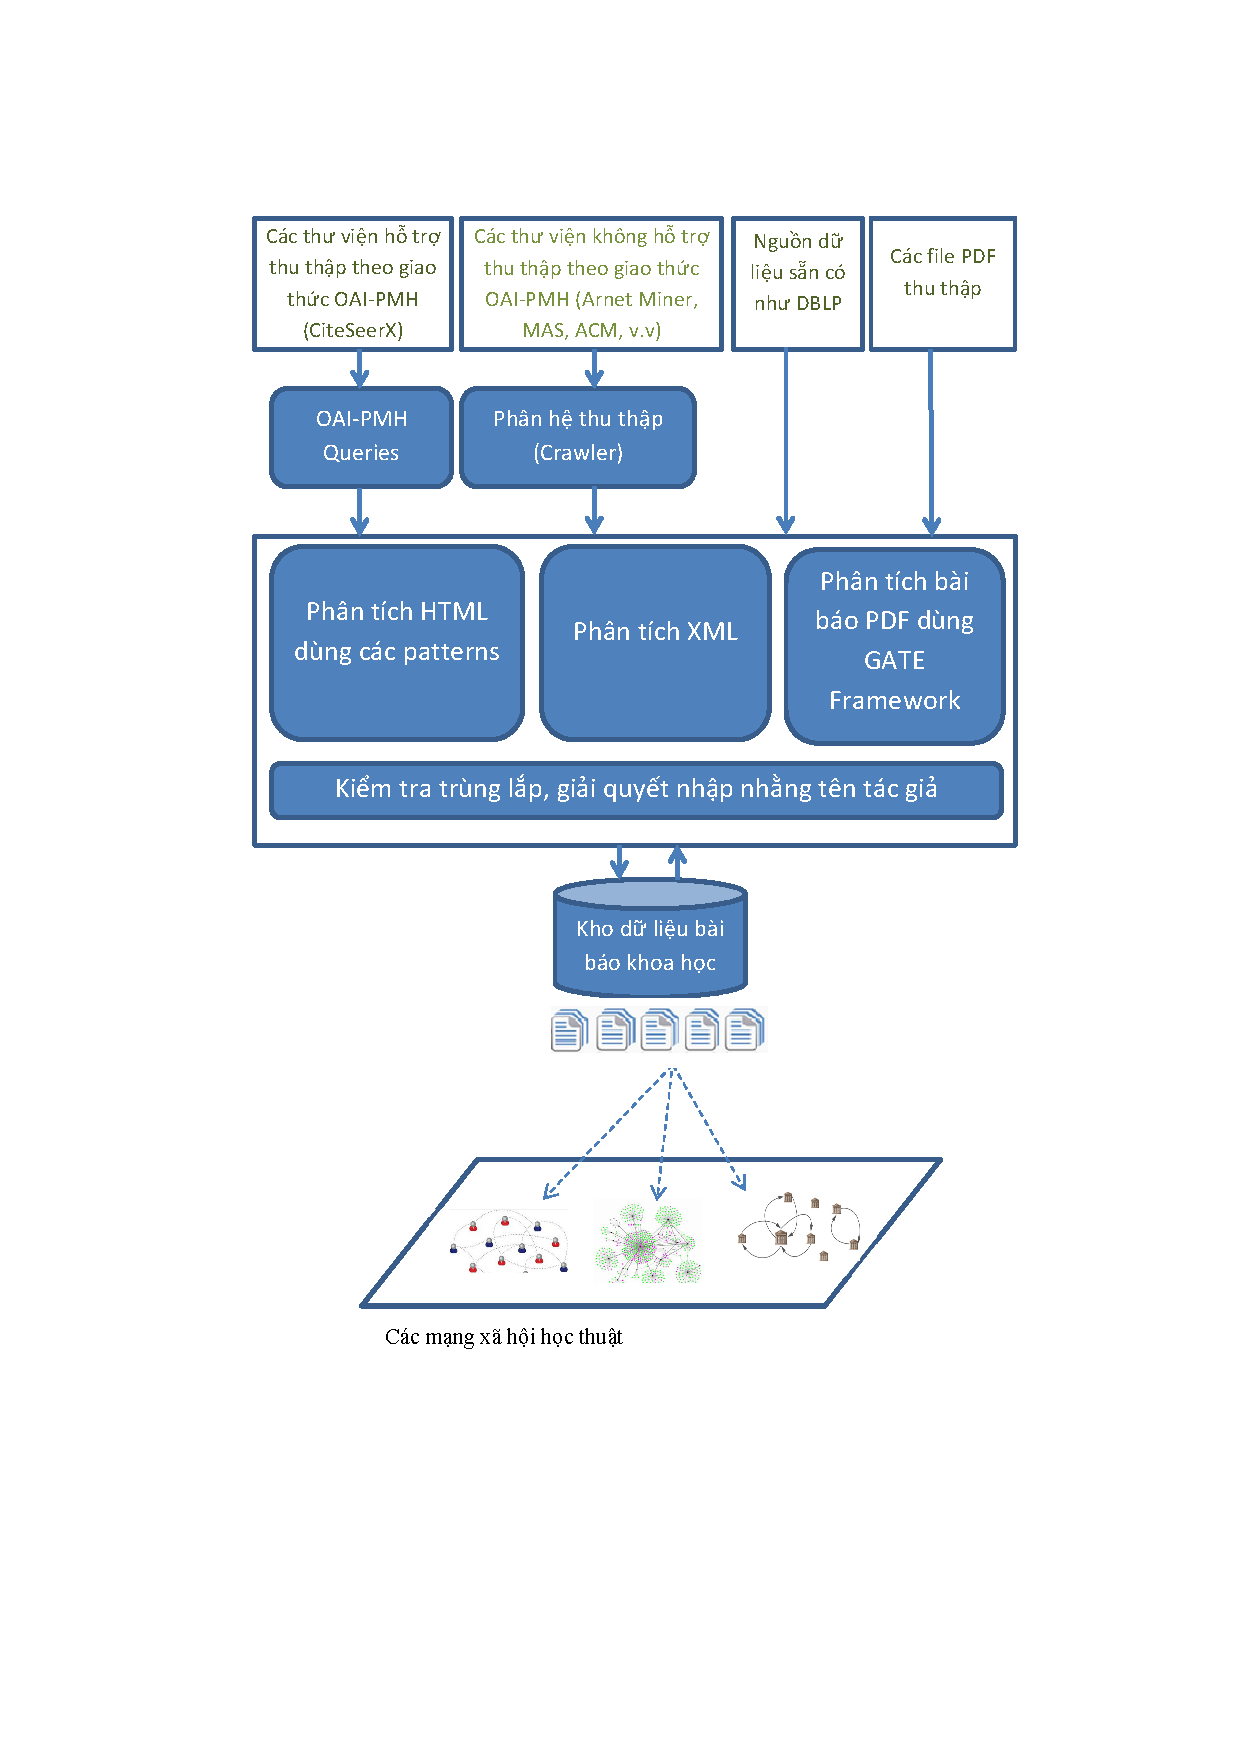
\includegraphics[width=0.65\textwidth]{Figure_A_1_.pdf}
%  \caption{Các mạng xã hội học thuật được rút trích và xây dựng từ kho dữ liệu bài báo}\label{fig:figure_A_1}
%\end{center}
%\end{figure}
%
%\section*{A.1 Tích hợp dữ liệu bài báo khoa học từ nhiều nguồn}
%Mỗi thư viện số sở hữu một cơ sở dữ liệu và một nguồn thông tin riêng dựa vào nguồn và cách họ thu thập. Vì vậy đôi khi một tài liệu, nghiên cứu viên hoặc các thông tin liên quan đến bài báo, nghiên cứu viên có thể tìm thấy trong thư viện này, nhưng không thấy trong thư viện kia. Để có một nguồn thông tin đầy đủ và phong phú phục vụ cho xây dựng, phân tích các mạng xã hội học thuật, chúng tôi đã tiến hành nghiên cứu phương pháp và xây dựng công cụ cho việc tích hợp dữ liệu khoa học từ nhiều nguồn không đồng nhất.
%
%Những nguồn dữ liệu khoa học được xem xét thu thập như: các bài báo khoa học dạng PDF, một số cơ sở dữ liệu khoa học và thư viện số trong lĩnh vực học thuật. Các hệ thống này có thể phân thành hai nhóm chính: (1) Nhóm hệ thống `mở' như DBLP, CiteSeerX, ArnetMiner là nhóm cho phép download miễn phí các bài báo mà họ đã lập chỉ mục (nếu có dữ liệu) (2) Nhóm thu phí truy cập, bao gồm các hệ thống thư viện số như ACM, IEEE Explore, Elsevier, SpringerLink. Phần bên dưới là kiến trúc hệ thống và giải pháp mà luận án áp dụng để xây dựng công cụ tích hợp các nguồn dữ liệu học thuật. 
%
%\subsection*{A.1.1 Kiến trúc hệ thống}
%\begin{figure}[h!]
%\begin{center}
%\advance\leftskip-3cm
%\advance\rightskip-3cm
%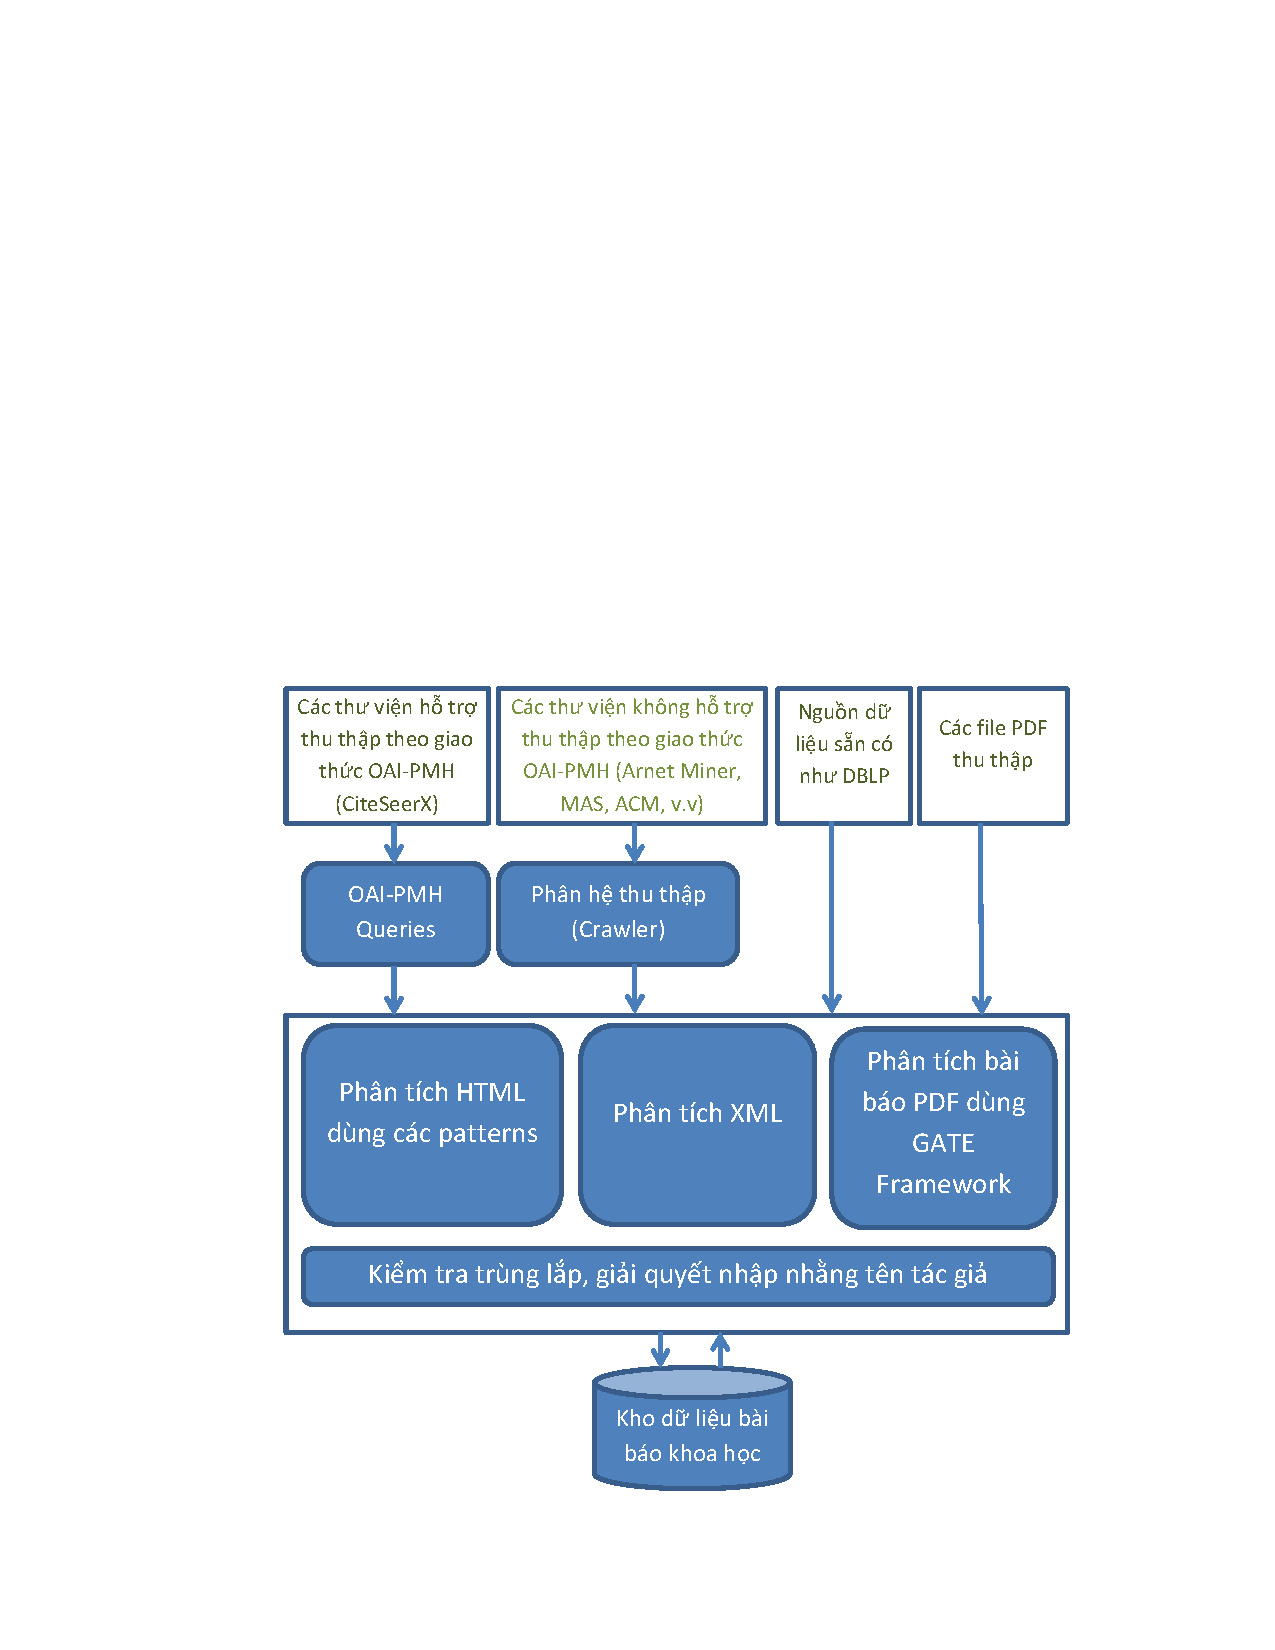
\includegraphics[width=0.7\textwidth]{Figure_A_2.pdf}
%\caption{Kiến trúc hệ thống tích hợp dữ liệu bài báo khoa học từ nhiều nguồn không đồng nhất}
%\label{fig:figure_A_2}
%\end{center}
%\end{figure}
%
%Hệ thống bao gồm các phân hệ chính sau:
%\begin{itemize}
%\item Rút trích metadata từ bài báo dạng PDF. Với những tính năng xử lý văn bản, ngôn ngữ tự nhiên mạnh mẽ của GATE framework, luận án dùng GATE Framework để định nghĩa các luật cho việc rút trích metadata từ các tập tin bài báo dạng PDF.\footnote{http://gate.ac.uk/, truy cập lần cuối ngày 07/02/2014}
%\item Phân hệ thu thập (Crawler): thu thập, rút trích thông tin bài báo từ các thư viện số trên internet. Phân hệ sẽ lập lịch, định thời và gởi các request đến các trang web của các thư viện số. Sau đó sẽ tiến hành phân tích các trang HTML trả về để rút trích ra các bài báo và metadata của nó. Với những thư viện số có hỗ trợ giao thức truy cập OAI-PMH thì hệ thống sẽ gởi các truy vấn OAI-PMH để rút trích metadata của các bài báo khoa học từ những thư viện số này.
%\item Xử lý dữ liệu có sẵn từ DBLP: phân hệ sẽ phân tích file dữ liệu của DBLP dưới dạng XML được công bố trên internet và import vào trong Cơ sở dữ liệu của hệ thống. 
%\item Xử lý nhập nhằng tên tác giả. Để đảm bảo tính nhất quán trong kho dữ liệu tích hợp, luận án cũng tiến hành nghiên cứu và xây dựng phân hệ giải quyết nhầp nhằng tên tác giả.
%\end{itemize}
%
%Kiến trúc trực quan của hệ thống tích hợp thông tin bài báo từ niều nguồn không đồng nhất thể hiện trong hình \ref{fig:figure_A_2}
%\subsection*{A.1.2 Rút trích metadata từ bài báo PDF}
%\subsubsection*{A.1.2.1 Đề xuất dùng luật dựa trên GATE Framework}
%GATE framework, một framework khá phổ biến cung cấp nhiều từ điển, ontologies, thư viện, công cụ cho xử lý văn bản, ngôn ngữ tự nhiên. Vì tính phổ biến, và những hỗ trợ mạnh mẽ của GATE cho xử lý văn bản, luận án quyết định chọn GATE để xây dựng các luật, mẫu để rút trích các metadata cho các tài liệu khoa học.
%\subsubsection*{A.1.2.2 Rút trích metadata cho mục Header và mục Reference}
%\begin{figure}[h]
%\begin{center}
%\advance\leftskip-3cm
%\advance\rightskip-3cm
%  % Requires \usepackage{graphicx}
%  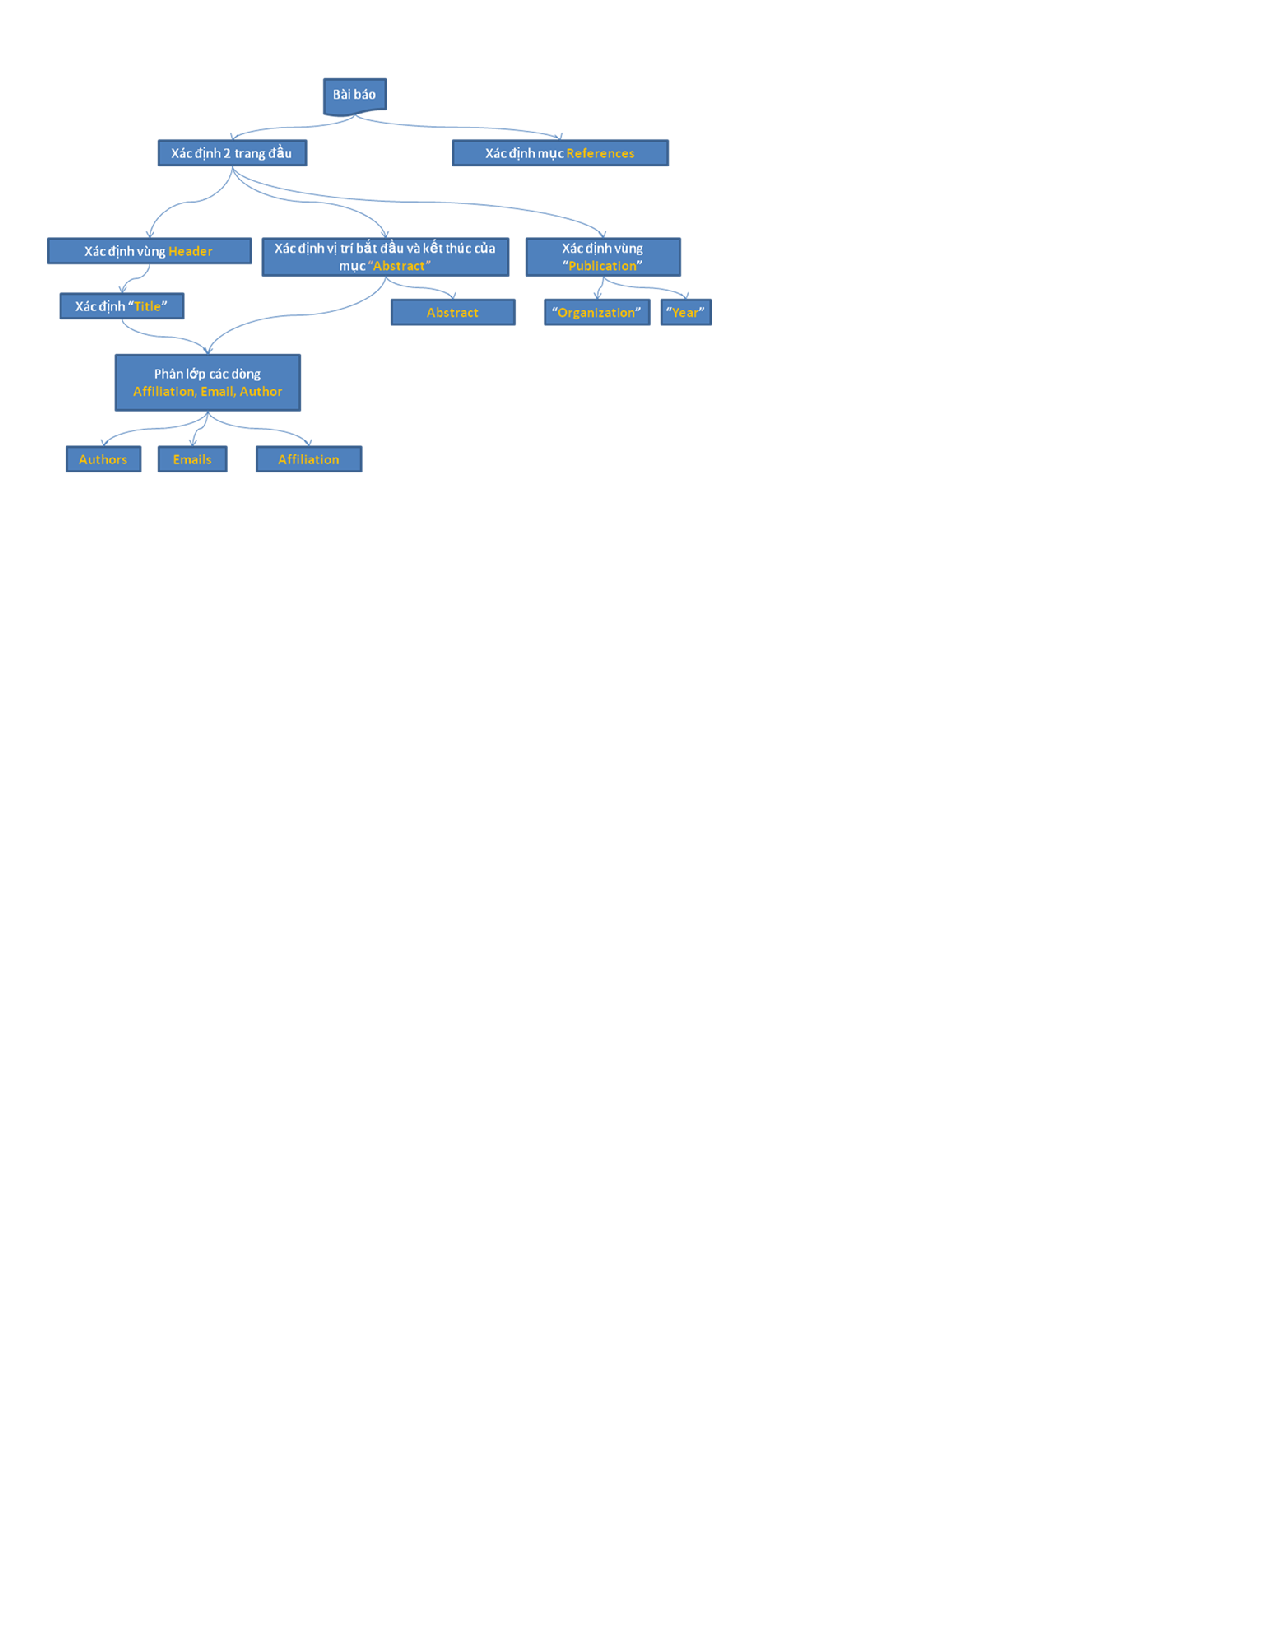
\includegraphics[width=0.99\textwidth]{Figure_A_3.pdf}
%  \caption{Các bước rút trích metadata từ header của bài báo}\label{fig:figure_A_3}
%\end{center}  
%\end{figure}
%Để rút trích metadata từ các bài báo dưới dạng PDF, chúng tôi tiến hành phân tích phần header và reference của bài báo. Đầu tiên tập tin PDF được chuyển thành tập tin dạng văn bản (text). Sau đó việc phân tích mục header và mục reference được thực hiện như mô tả chi tiết trong hình \ref{fig:figure_A_3} và hình \ref{fig:figure_A_4}. 
%\begin{figure}[ht]
%\begin{center}
%\advance\leftskip-3cm
%\advance\rightskip-3cm
%  % Requires \usepackage{graphicx}
%  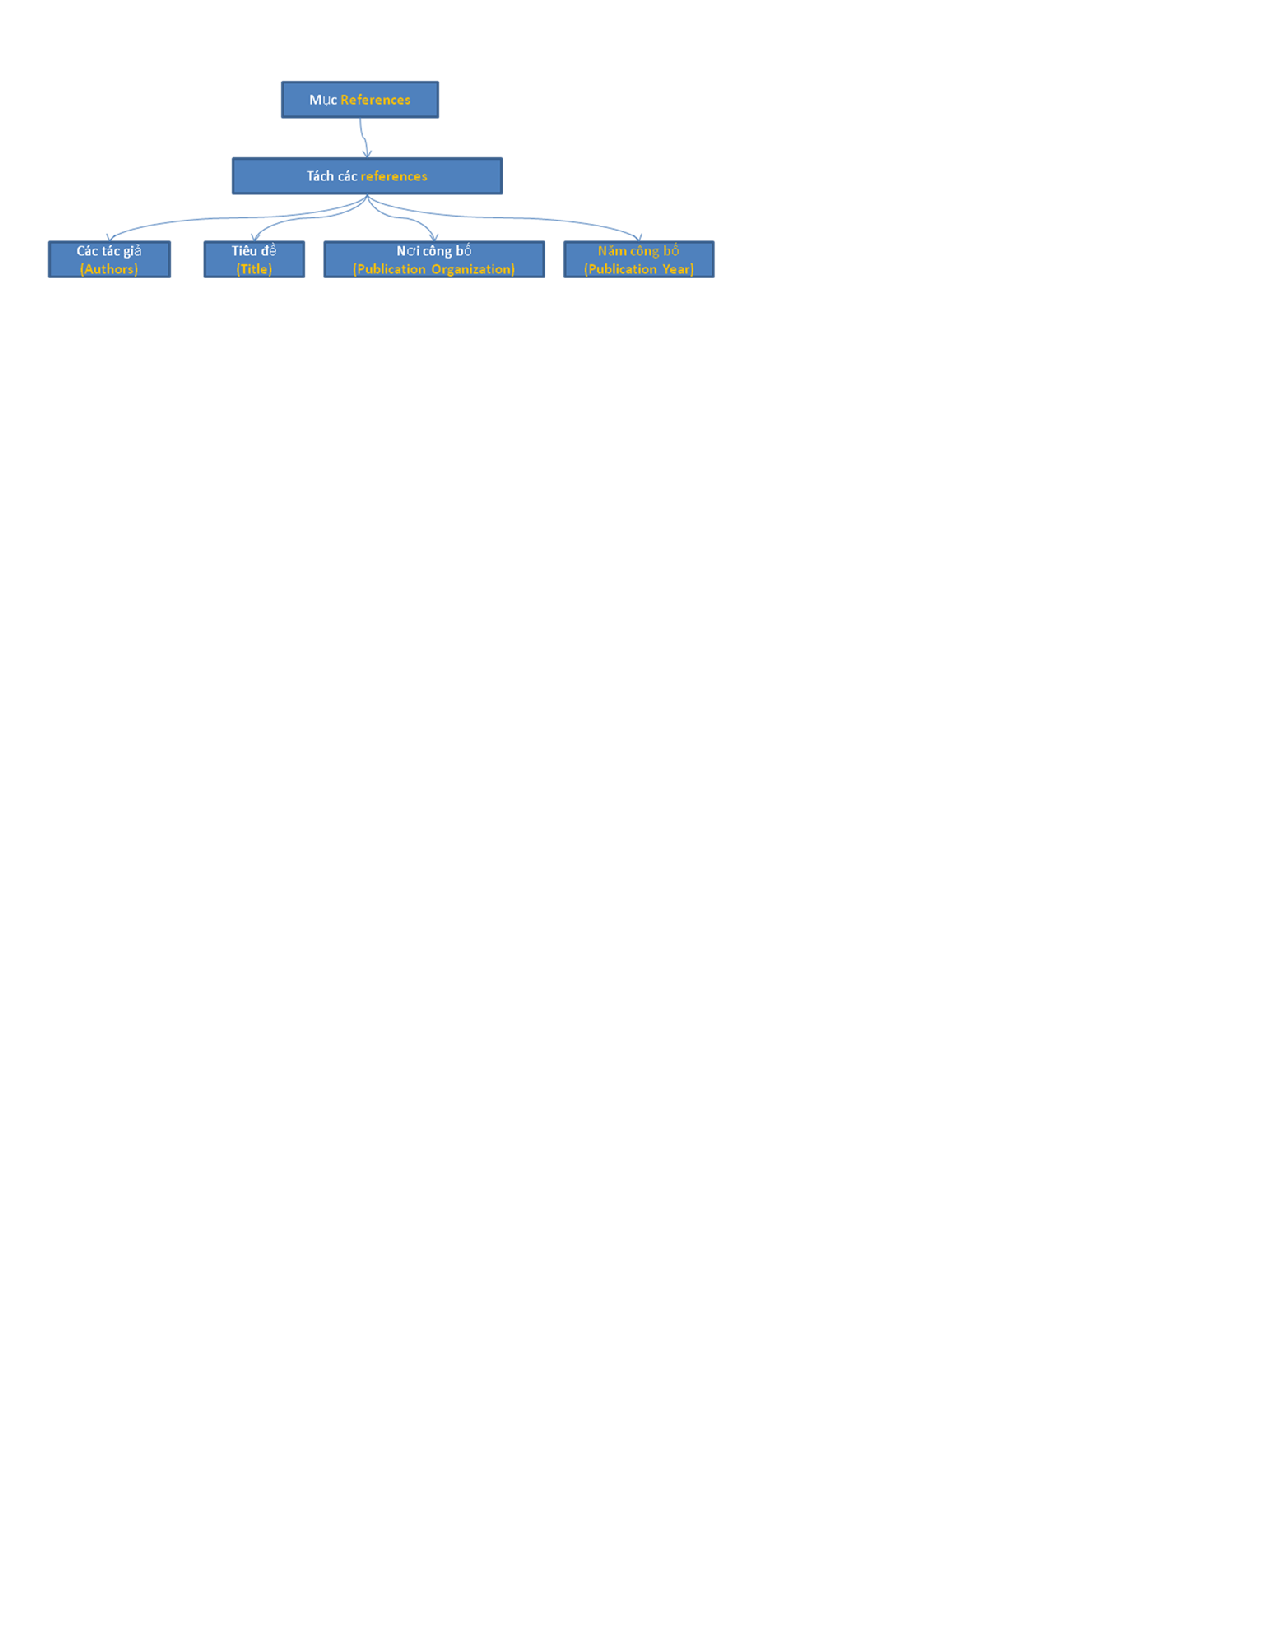
\includegraphics[width=0.99\textwidth]{Figure_A_4.pdf}
%  \caption{Các bước rút trích metadata từ phần reference của bài báo}\label{fig:figure_A_4}
%\end{center}  
%\end{figure}

\section*{A.1 Các luật JAPE để rút trích thông tin từ bài báo khoa học PDF}
\subsubsection*{Luật JAPE để xác định tên tác giả}
\begin{lstlisting}[frame=single]
Rule: Author
(
	(
		{Person} | 
		( 
			{Token.string!=",", 
			Token.string!="and", 
			Token.kind!="number"}
		)+
	):author
)
-->
:author.Author = {rule= "Author"}
\end{lstlisting}

\subsubsection*{Luật JAPE để xác định các `Email'}
\begin{lstlisting}[frame=single]
Rule:LineEmailAnnotation
(	(
		{Token.string=="{"}
		(
			{Token}
			({SpaceToken.kind=="space"})?
		)+
		({SpaceToken.kind=="control"})?
	)?
	(
		{Token}
		({SpaceToken.kind=="space"})?
	)+
	(
		{Token.string=="@"} | 
		{Address.kind=="email"} | 
		{Token.string=="}"}
	)
	({SpaceToken.kind=="space"})?
	(
		{Token}
		({SpaceToken.kind=="space"})?
	)+
):lineEmailAnnotation
-->
:lineEmailAnnotation.LineEmailAnnotation = 
{rule = "LineEmailAnnotation"}
\end{lstlisting}

\subsubsection*{Luật JAPE để xác định cơ quan công tác `Affiliation'}
\begin{lstlisting}[frame=single]
Rule:LineAffiliationAnnotation
((	{Token.string=="Dept"} | 
	{Token.string=="dept"} |
	{Token.string=="University"} | 
	{Token.string=="university"} |
	{Token.string=="Faculty"} | 
	{Token.string=="FACULTY"} |
	{Lookup.majorType=="location"}  |
	{Lookup.majorType=="org_key"} | 
	{Lookup.majorType=="org_base"} |
	{Lookup.majorType=="cdg"} | 
	{Lookup.majorType=="facility_key", 
	!Token.string=="Hall"} |
	((	{Token.kind=="number", Token.length>=3}
		{SpaceToken.kind=="space"}
	 ) |
	 (	{Token.kind=="number"}
		({SpaceToken.kind=="space"})?
		({Token.kind== "punctuation", 
			Token.subkind == "dashpunct"})
		({SpaceToken.kind=="space"})?
		{Token.kind=="number"}
	 )
	)
 )
 ({SpaceToken.kind=="space"})?
 (	{Token}
	({SpaceToken.kind=="space"})?
 )*
):lineAffiliationAnnotation
-->
:lineAffiliationAnnotation.LineAffiliationAnnotation = 
{rule = "LineAffiliationAnnotation"}
\end{lstlisting}

\subsubsection*{Luật JAPE để xác định vùng `Abstract'}
\begin{lstlisting}[frame=single]
Rule: AbstractKeyword
(   
	({SpaceToken.kind=="control"})+
	(	{Token.string=="Abstract."} | 
		{Token.string=="ABSTRACT."} |
		{Token.string=="Abstract"} | 
		{Token.string=="ABSTRACT"}
	)
	({Token.string=="."})?
):abstract_Keyword 
-->
:abstract_Keyword.AbstractKeyword = 
{rule = "AbstractKeyword"} 
\end{lstlisting}

\subsubsection*{Luật JAPE để xác định, tách vùng `Reference'}
\begin{lstlisting}[frame=single]
Rule: ReferencesKeyword
(
	({SpaceToken.kind=="control"})+
	(
		{Token.kind=="number"}
		({Token.string=="."})?
		({SpaceToken.kind=="space"})+
	)?
	(	{Token.string=="References"} | 
		{Token.string=="REFERENCES"} | 
		{Token.string=="reference"} | 
		{Token.string=="REFERENCE"} 
	)
):referencesKeyword 
-->
:referencesKeyword.ReferencesKeyword = 
{rule= "ReferencesKeyword" }
\end{lstlisting}

%\subsection*{A.1.3 Thu thập, rút trích metadata từ các trang web}
%Công cụ của chúng tôi hỗ trợ thu thập, rút trích metadata của các bài báo từ những trang web thư viện điện tử theo hai phương thức: (1) truy vấn từ các thư viện điện tử hỗ trợ giao thức OAI-PMH như CiteSeerX\footnote{http://csxstatic.ist.psu.edu/about/data, truy cập lần cuối ngày 07/02/2014}, ArXiv\footnote{http://arxiv.org, truy cập lần cuối ngày 07/02/2014}; (2) thu thập, rút trích từ cách trang không hỗ trợ OAI-PMH.
%
%Với các thư viện hỗ trợ OAI-PMH, chúng tôi xây dựng các mẫu truy vấn liên quan đến các động từ được định nghĩa trong OAI-PMH để thu thập được dữ liệu. Ví dụ các mẫu truy vấn được gởi đến CiteSeerX được định nghĩa trong bảng \ref{tab:table_A_1}.
%\begin{table}[ht]
%\begin{center}
%    \caption{Các mẫu truy vấn được gởi đến CiteSeerX}\label{tab:table_A_1}
%    \begin{tabular}{p{7.5cm}|p{6.5cm}}
%    \hline
%    Mẫu truy vấn & Mô tả \\  
%    \hline
%    $http://citeseerx.ist.psu.edu/oai2?verb=Identify$ & The query to CiteSeerX to retrieve information about the repository.\\
%    \hline
%    $http://citeseerx.ist.psu.edu/oai2?verb=ListMetadataFormats$ & The query to CiteSeerX to retrieve the metadata formats available from the repository. \\
%    \hline
%    $http://citeseerx.ist.psu.edu/oai2?verb=ListRecords\&metadataPrefix=oai\_dc$ & The query to CiteSeerX to harvest records. \\
%    \hline 
%    $http://citeseerx.ist.psu.edu/oai2?verb=ListIdentifiers\&metadataPrefix=oai\_dc\&from=1900-01-01\&until=2013-01-01$ & The query to CiteSeerX to retrieve metadata record formatted Dublin Core, published from 1900-01-01 and until 2013-01-1. \\
%    \hline
%    \end{tabular}
%\end{center}
%\end{table}
%
%Đối với các thư viện số không hỗ trợ OAI-PMH, các yêu cầu đến các trang web này dưới dạng một câu truy vấn tìm kiếm có đầu vào là một từ khóa. Những từ khóa tìm kiếm lấy từ danh sách phân lọai chuyên ngành Khoa học Mát tín của ACM. Bảng \ref{tab:table_A_2} mô tả các mẫu câu truy vấn được hình thành và gởi đến một số thư viện số phổ biến. Sau khi gởi các truy vấn đến các thư viện số, kết quả trả về là dưới dạng HTML. Hệ thống sẽ tiến hành phân tích các trang HTML trả về này để rút trích ra metadata tương ứng của các bài báo khoa học.
%
%\begin{table}[ht]
%\centering
%    \caption{Các mẫu truy vấn được gởi đến các thư viện không hỗ trợ OAI-PMH tương ứng với từ khóa 'Information Extraction'}\label{tab:table_A_2}
%    \begin{tabular}{p{2.5cm} | p{10.5cm}}
%    \hline
%    Thư viện số & Mẫu truy vấn\\  
%    \hline
%    ACM & $http://portal.acm.org/results.cfm?query=information\%20extraction\&dl=ACM\&coll=Portal\&short=0$\\
%    \hline
%    IEEE Xplore & $http://ieeexplore.ieee.org/search/freesearchresult.jsp$?$reload=true\&queryText=information\%20extraction$\\
%    \hline
%    MAS & $http://academic.research.microsoft.com/Search?query=Information\%20Extraction\&SearchDomain=2$\\
%    \hline
%    \end{tabular}
%\end{table}

\section*{A.2 Giải quyết nhập nhằng tên tác giả cho kho bài báo tích hợp}
Bài toán nhập nhằng tên tác giả là vấn đề đã và đang thu hút nhiều quan tâm nghiêm cứu trong lĩnh vực thư viện số cũng như các hệ thống tìm kiếm tài liệu, chuyên gia. Nhập nhằng tên tác giả xảy ra khi: một tác giả sử dụng nhiều bút danh khác nhau (synonyms), hoặc nhiều tác giả khác nhau nhưng có cùng bút danh (polysems) trong các bài báo khoa học \cite{Ferreira:2012:BSA:2350036.2350040}. Thông thường những tác giả người Châu Á rất dễ bị nhầp nhằng tên, lý do chính là thứ tự trong cách viết họ tên. Bình thường thì họ viết họ trước, tên sau. Đôi khi tên đứng trước, họ đứng sau và tên lót (middle name) có lúc được dùng, có lúc không.
Bảng \ref{tab:table_A_3} trình bày một ví dụ minh họa về trường hợp nhập nhằng tên tác giả trong kho dữ liệu bài báo khoa học. Tên tác giả \textbf{\textit{`Tuan Nguyen'}} trong bài báo số 1 và \textbf{\textit{`Anh-Tuan Nguyen'}} trong bài báo số 3 là cùng một người (synonyms); Trong khi tác giả \textbf{\textit{`Tuan Nguyen'}} trong bài số 1 và \textbf{\textit{`Tuan Nguyen'}} trong bài số 2 là hai người khác nhau (polysems). 
\begin{table}[ht]
\centering
    \caption{Ví dụ các bài báo nhập nhằng tên tác giả}\label{tab:table_A_3}
    \begin{tabular}{ p{0.8cm} | p{12.9cm}}
    \hline
     \centering \textbf{STT} & \textbf{Bài báo}\\
    \hline
     \centering \multirow{4}{*}{1} & Multiagent Place-Based Virtual Communities for Pervasive Computing. \\
     & Conference: PERCOM '08 Proceedings of the 2008 Sixth Annual IEEE International Conference on Pervasive Computing and Communications. \\
     & Authors: \textbf{\textit{Tuan Nguyen}}, Seng Loke; Torabi, T.; Hongen Lu.\\
     & Dept. of Comput. Sci. \& Comput. Eng., La Trobe Univ., Bundoora, VIC.\\
    \hline
    \centering \multirow{4}{*}{2} & Stationary points of a kurtosis maximization algorithm for blind signal separation and antenna beamforming. \\   
    & Journal: Journal IEEE Transactions on Signal Processing \\
    & Authors: Zhi Ding, \textbf{\textit{Tuan Nguyen}}\\
    & Dept. of Electr. \& Comput. Eng., Iowa Univ., Iowa City, IA.\\
    \hline
    \centering \multirow{4}{*}{3} & Semantic-PlaceBrowser: Understanding Place for Place-Scale Context-Aware Computing \\   
	& Conference: The Eighth International Conference on Pervasive Computing (Pervasive 2010), Helinski, Finland, 2010. \\
    & Authors: Authors: \textbf{\textit{Anh-Tuan Nguyen}}, Seng Wai Loke, Torab Torabi, Hongen Lu.\\
    & Department of Computer Science and Computer Engineering, La Trobe University, Victoria, 3086, Australia\\
    \end{tabular}
\end{table}

Phần bên dưới sẽ trình cách tiếp cận và đóng góp của luận án đối với với đề giải quyết nhầp nhằng tên tác giả khi tích hợp dữ liệu khoa học từ nhiều nguồn không đồng nhất.

\subsection*{A.2.1 Tiếp cận đề xuất}
Làm thế nào để giải quyết nhập nhằng tên tác giả trong 2 bài báo khác nhau. \cite{Ferreira:2012:BSA:2350036.2350040} đã phân các phương pháp thành hai nhóm chính: (1) gom nhóm các bài báo của cùng một tác giả bằng các phương pháp tính toán tương tự (học tính synonyms hay polysems của hai bài báo); (2) Học và xây dựng mô hình hồ sớ cá nhân (profile) cho mỗi tác giả, và gán những bài báo tương ứng với tác giả nào đó dựa trên mô hình đã học. Cả hai cách tiếp cận này đều có gắng xác định tập đặc trưng dựa trên sự tương tự của các thuộc tính metadata rút trích từ các bài báo khoa học. Tập đặc trưng sẽ khác nhau tùy thuộc vào đặc tính của tập dữ liệu thực nghiệm. Với các dữ liệu thu thập từ nhiều nguồn không đống nhất, luận án đã tiếp cận dùng phương pháp học giám sát và đề xuất tập đặc trưng để giải quyết vấn đề nhập nhằng tên giữa hai bài báo khác nhau.
\subsubsection*{A.2.1.1 Các phương pháp so khớp chuỗi phổ biến}
\citet{Bilenko:2003:ANM:1137237.1137369}, \citet{CohenRF03}, đã khảo sát các độ đo, phương pháp tính toán sự tương tự của hai chuỗi ký tự nhằm xác định sự trúng lắp. Các độ đo này cơ bản được chia thành 3 nhóm chính: (1) Khoảng cách biến đổi (Edit distance); (2) Tương tự dựa trên từ (token); và (3) Độ đo kết hợp giữa từ và khoảng cách biến đổi.

\subsubsection*{Khoảng cách biến đổi (Edit Distance)} 
Khoảng cách biến đổi giữa chuỗi X và chuỗi Y là chi phí những thao tác thay đổi mà có thể chuyển chuỗi X thành chuỗi Y. Một số độ đo khoảng cách biến đổi phổ biến như Levenshtein, Monger-Elkan, Jaro, Jaro-Winkler \cite{CohenRF03}. Levenshtein được biết đến như độ đo khoảng cách biến đổi phổ biến nhất. Với độ đo Levenshtein, chi phí biến đổi chuỗi ký tự được tính bởi 3 loại thao tác: (1) Thao tác chèn một ký tự mới; (2) Thao tác xóa một ký tự; (3) Thao tác thay thế một ký tự bằng một ký tự khác.
\begin{equation}
Sim_{levenshtein}(X,Y) = 1 - \displaystyle\frac{d(X,Y)}{[max(length(X), length(Y))]}
\end{equation}
Trong đó,
\begin{itemize}
\item $d(X,Y)$: Số thao tác biến đổi tối thiểu để chuyển chuỗi X thành chuỗi Y.
\item $length(x)$: Chiều dài chuỗi X.
\end{itemize}

\subsubsection*{Tương tự dựa trên từ (token)} 
Trong một số trường hợp thì thứ tự của từ không thật sự quan trọng. Khi đó hệ số Jaccard và TF-IDF là những độ đo dựa trên từ hiệu quả và được dùng phổ biến \cite{Baeza-Yates:1999:MIR}, \cite{CohenRF03}.
\begin{equation}
Sim_{jaccard}(X,Y) = \displaystyle\frac{|X \bigcap Y|}{|X \bigcup Y|}
\end{equation}
\begin{itemize}
\item $|X \bigcap Y|$: Số lượng từ giống nhau giữa chuỗi X và chuỗi Y.
\item $|X \bigcup Y|$: Số lượng từ phân biệt nhau đôi một trong cả chuỗi X và chuỗi Y.
\end{itemize}

\subsubsection*{Đo đo kết hợp} 
Một độ đo phổ biến cho sự kết hợp là độ đo Mogne-Elkan \cite{CohenRF03}. Với độ đo Mogne-Elkan, hai chuỗi X, Y sẽ được tách thành các chuỗi con dưới dạng các từ là  $X = x_{1}...x_{K}$ và $Y = y_{1}...y_{L}$. Khoảng cách biến đổi sẽ được tính cho mỗi từ trong chuỗi con. Cụ thể Độ đo Mogne-Elkan được tính như sau:
\begin{equation}
Sim_{monge-elkan}(X,Y) = \displaystyle\frac{1}{K}\sum_{i=1}^K \max_{j=1}^{L} Sim^{'} (x_{i},y_{j})
\end{equation}
Trong đó,
\begin{itemize}
\item $Sim^{'}$: là khoảng cách biến đổi (Edit Distance) như Levenshtein.
\end{itemize}

\subsubsection*{A.2.1.2 Đề xuất tập đặc trưng} \label{section:ProposedFeatureSet}
Với bài toán nhập nhằng tên tác giả trong kho dữ liệu tích hợp, các chuỗi metadata của bài báo khoa học cần xem xét đó là: tên tác giả, tên đồng tác giả, tên cơ quan công tác, độ tương tự của các từ khóa trong bài báo. Với các chuỗi metadata này thì những độ đo tương tự ở mức từ, không quan tâm đến thứ tự của từ trong chuỗi là phù hợp, chẳng hạn như Jaccard. Các độ đo khoảng cách biến đổi (edit distance) thông thường chỉ phù hợp cho việc kiểm tra lỗi đánh máy nhầm. Do đó, luận án đã dùng Jaccard để tính toán độ tương tự của các metadata trong hai bài báo khoa học. Bên dưới là tập đặc trưng và cách tính để giải giải quyết nnập nhằng tên tác giả bằng phương pháp học giám sát.

\subsubsection*{(1) Tên tác giả}
Chúng ta đưa ra giả thuyết: `Nếu hai chuỗi tên tác giả càng tương tự thì khả năng hai chuỗi này liên quan đến một người càng cao'. Độ tương tự hai chuỗi tên tác giả được tính như sau:
\begin{equation}
Author\_Name\_Sim(A,B) = \displaystyle\frac{|Author\_Name\_A \bigcap Author\_Name\_B|}{|Author\_Name\_A \bigcup Author\_Name\_B|} 
\end{equation}
Trong đó,
\begin{itemize}
\item $Author\_Name\_A$: Tên tác giả A trong bài báo đang xét.
\item $|A \bigcap B|$: Số lượng từ giống nhau giữa tên tác giả A và B.
\item $|A \bigcup B|$: Số lượng từ đôi một khác nhau trong tên của A và B.
\end{itemize}
Ví dụ:

\emph{Author\_Name\_A="Tuan Nguyen" và Author\_Name\_B="Nguyen Anh Tuan"}

\emph{$|Author\_Name\_A \bigcap Author\_Name\_B| = 2$}

$|Author\_Name\_A \bigcup Author\_Name\_B |= 3$, và

$Author\_Name\_Sim(A, B) \approx  0,67.$\\

\subsubsection*{(2) Tên đồng tác giả}
Trong trường hợp này, giả thuyết sẽ là: `Nếu hai tác giả nhập nhằng, có càng nhiều đồng tác giả cùng tên trong hai bài báo khác nhau thì khả năng hai người này là một càng cao'. Giá trị đặc trưng dựa trên độ tương tự đồng tác giả được tính như sau:
\begin{equation}
CoAuthors\_Names\_Sim(A,B) = MAX(Author\_Name\_Sim(A_{i},B_{j}))
\end{equation}
Trong đó,
\begin{itemize}
\item $A_{i}\in {CoAuthors(A)}$ \\
và CoAuthors(A): tập các đồng tác giả của $A$ trong bài báo  $P_{1}$.
\item $B_{j}\in {CoAuthors(B)}$ \\
và CoAuthors(B): tập các đồng tác giả của $A$ trong bài báo  $P_{2}$.
\end{itemize}

\subsubsection*{(3) Cơ quan Công tác của tác giả}
Cơ quan công tác của hai tác giả nhập nhằng trong hai bài báo khác nhau là một trong những đặc trưng quan trọng giúp nhận diện có hay không hai tác giả nhập nhằng này là một người. Độ tương tự cơ quan công tác của hai tác giả nhập nhằng cũng được tính dùng hệ số Jaccard như sau:
\begin{equation}
Aff\_Sim(A,B) = \displaystyle\frac{|Aff\_A \bigcap Aff\_B|}{|Aff\_A \bigcup Aff\_B|}
\end{equation}
Trong đó,
\begin{itemize}
\item $Aff\_A$: Cơ quan của $A$ trong bài báo đang xét.
\item $|Aff\_A \bigcap Aff\_B|$: Số lượng từ giống nhau giữa tên cơ quan của A và cơ quan của B.
\item $|Aff\_A \bigcup Aff\_B|$: Số lượng từ phân biệt đôi một trong tên cơ quan của A và tên cơ quan của B.
\end{itemize}

\subsubsection*{(4) Cơ quan Công tác của Đồng tác giả}
Giả thuyết được đưa ra trong trường hợp này là: 'Nếu hai tác giả nhập nhằng càng có nhiều đồng tác giả làm cùng cơ quan thì khả năng hai người này là một càng cao'. Giá trị đặc trưng này được tính như sau:
\begin{equation}
CoAuthor\_Affs\_Sim(A,B) = MAX(Aff\_Sim(Aff_{i}\_P{1},Aff_{j}\_P_{2}))
\end{equation}
Trong đó,
\begin{itemize}
\item $Aff_{i}\_P{1}\in {CoAuthors\_Affs(A)}$\\
i=1..n (n: số lượng đồng tác giả của A trong bài bái $P_{1}$) \\
và CoAuthors\_Affs(A): là các cơ quan của các đồng tác giả của $A$ trong bài báo $P_{1}$.
\item $Aff_{i}\_P{2}\in {CoAuthors\_Affs(B)}$\\
j=1..m (m: số lượng đồng tác giả của B trong bài báo $P_{2}$) \\
và CoAuthors\_Affs(B): là các cơ quan của các đồng tác giả của $B$ trong bài báo $P_{2}$.
\end{itemize}

\subsubsection*{(5) Từ khóa bài báo}
Hai bài báo liên quan đến hai tác giả nhập nhằng càng chứa nhiều từ khóa tương tự nhau, thì khả năng hai tác giả này là một người càng cao. Đặc trưng tương tự dựa trên từ khóa được tính như sau:
\begin{equation}
Paper\_Keywords\_Sim(A,B) \displaystyle\frac{|Paper\_Keywords\_A \bigcap Paper\_Keywords\_B|}{|Paper\_Keywords\_A \bigcup Paper\_Keywords\_B|}
\end{equation}
Trong đó,
\begin{itemize}
\item $Paper\_Keywords\_A$: tập các từ khóa trong bài báo A.
\item $|Paper\_Keywords\_A \bigcap Paper\_Keywords_B|$: số từ (token) giống nhau của các từ khóa trong bài báo A và bài báo B.
\item $|Paper\_Keywords\_A \bigcup Paper\_Keywords\_B|$: tổng số từ (token) đôi một khác nhau trong các từ khóa của bài báo A và bài báo B.
\end{itemize}

Với tập đặc trưng đề xuất, các vector tương ứng với hai bài báo có tác giả nhập nhằng được xây dựng. Luận án áp dụng các phương pháp học giám để học và nhận diện tác giả nhập nhằng dựa trên tập dữ liệu được gán nhãn cho huấn luyện và kiểm tra. 

%Thực nghiệm được tiến hành trên các phương pháp học giám sát như Bayesian Network, Support Vector Machine, Random Forest, ...
%\subsection*{A.2.2 Thực nghiệm và nhận định}
%Phần này trình bày việc đánh giá hiệu quả của tập đặc trưng đề xuất cho bài toán giải quyết nhập nhằng tên tác giả thông qua các phương pháp học giám sát như Random Forest, kNN, SVM, C4.5, Bayes Network. Kết quả thực nghiệm nhằm cho biết hiệu quả của tập đặc trưng, cũng như bộ phân lớp phù hợp.
%\subsubsection*{Tập dữ liệu}
%Với kho dữ liệu thu thập và tích hợp từ nhiều nguồn không đồng nhất, luận án lọc ra một tập con liên quan đến 10 tác giả là người Việt Nam để tiến hành thực nghiệm. Với mỗi tác giả, chọn ra 30 bài báo trong kho dữ liệu thu thập từ nhiều nguồn (chứa các tác giả nhập nhằng). Tập dữ liệu huấn luyện và kiểm tra được xây dựng bằng cách bắt cặp trong 30 bài báo được cho là liên quan đến một tác giả. Dựa trên hiểu biết của mình, chúng tôi đã gán nhãn cho mỗi cặp bài báo là 1 nếu cùng liên quan đến một tác giả, ngược lại là 0. Tổng cộng chúng tôi có 4350 mẫu trong tập dữ liệu của mình. Bảng \ref{tab:table_2_4} trình bày chi tiết về tập dữ liệu chuẩn bị cho thực nghiệm. Mỗi mẫu dữ liệu liên quan đến một cặp bài báo chứa các tác giả nhập nhằng và mỗi mẫu này sẽ được mã hóa bằng một vector đặc trưng. Trọng số của các đặc trưng được tính như đã trình bày trong mục \ref{section:ProposedFeatureSet}.
%
%\begin{table}
%\centering
%    \caption{Tập dữ liệu thực nghiệm được gán nhãn cho huấn luyện và kiểm tra}\label{tab:table_2_4}
%    \begin{tabular}{p{4.0cm}|p{2.0cm}|p{1.9cm}|p{1.9cm}|p{1.9cm}}
%    \hline
%    Tên tác giả & Số bài báo liên quan & Số cặp gán nhãn & Số cặp gán nhãn 0 & Số cặp gán nhãn 1 \\
%    \hline
%    Kiem Hoang & 30 & 435 & 25 & 410 \\
%    Ho Tu Bao & 30 & 435 & 0 & 435 \\
%    Nguyen Ngoc Thanh & 30 & 435 & 141 & 294 \\
%    Phan Thi Tuoi & 30 & 435 & 0 & 435 \\
%    Ha Quang Thuy & 30 & 435 & 84 & 351 \\
%    Le Hoai Bac & 30 & 435 & 0 & 435 \\
%    Duong Anh Duc & 30 & 435 & 29 & 406 \\
%    Cao Hoang Tru & 30 & 435 & 26 & 409 \\
%    Dinh Dien & 30 & 435 & 51 & 384 \\
%    Le Dinh Duy & 30 & 435 & 57 & 378 \\
%    \hline
%    \end{tabular}
%\end{table}
%
%\subsubsection*{Kết quả thực nghiệm \& Nhận định}
%Luận án đã kiểm tra với 5 phương pháp học giám sát kNN, Support Vector Machine, Random Forest, C4.5, Bayes Network. Phần mềm khai thác dữ liệu và máy học Weka được dùng để huấn luyện và đánh giá hiệu quả của tập đặc trưng cũng như xem xét bộ phân lớp phù hợp.
%
%Chúng tôi áp dụng phương pháp đánh giá chéo 10-fold (10-fold cross validation). Tức tập dữ liêu sẽ được chia nhỏ thành 10 tập con với kích thước như nhau. Quá trình đánh giá chéo được lặp 10 lần, mỗi lần lặp thì một tập con được dùng để kiểm tra, còn các tập con còn lại dùng để huấn luyện. Như vậy mỗi tập con sẽ được dùng chính xác một lần với vai trò là dữ liệu kiểm tra (validation data). Kết quả thực nghiệm đánh giá chéo qua 10-fold với tập đặc trưng đề xuất và các bộ phân lớp giám sát được thể hiện trong bảng \ref{tab:table_2_5}
%
%\begin{table}
%\centering
%    \caption{Kết quả thự nghiệm và đánh giá chéo với 10-fold}\label{tab:table_2_5}
%    \begin{tabular}{p{4.3cm}|p{1.6cm}|p{1.6cm}|p{1.6cm}|p{1.6cm}|p{1.6cm}}
%    \hline    
%	Đánh giá chéo 10-fold & kNN & Random Forest & C4.5 & SVM & Bayesian Network \\
%    \hline
%    Độ chính xác fold-1 & 90.57 & 90.57 & 90.34 & 88.05 & 75.63 \\
%    Độ chính xác fold-2 & 89.20 & 89.20 & 88.51 & 87.59 & 80.00 \\
%    Độ chính xác fold-3 & 94.02 & 93.79 & 91.72 & 88.51 & 82.99 \\
%    Độ chính xác fold-4 & 95.86 & 93.56 & 95.86 & 92.87 & 79.08 \\
%    Độ chính xác fold-5 & 98.16 & 98.16 & 98.39 & 97.93 & 74.71 \\
%    Độ chính xác fold-6 & 97.24 & 96.78 & 97.24 & 95.63 & 86.21 \\
%    Độ chính xác fold-7 & 95.17 & 95.63 & 96.32 & 93.79 & 86.90 \\
%    Độ chính xác fold-8 & 95.40 & 95.17 & 95.63 & 91.72 & 85.29 \\
%    Độ chính xác fold-9 & 94.25 & 94.25 & 94.71 & 94.94 & 88.05 \\
%    Độ chính xác fold-10 & 95.63 & 95.17 & 91.03 & 88.05 & 76.78 \\
%    \hline
%    Độ chính xác trung bình & 94.55 & 94.23 & 93.98 & 91.91 & 81.56 \\
%    \hline
%    \end{tabular}
%\end{table}
%
%Hình \ref{fig:figure_A_5} trực quan việc so sánh độ chính xác dùng các bộ phân lớp khác nhau đối với tập đặc trưng đề xuất cho bài toán nhập nhằng tên tác giả. Kết quả thực nghiệm cho thấy với tập dữ liệu của bài toán này thì bộ phân lớp Random Forest, kNN, C4.5 cho kết quả trội hơn các bộ phân lớp khác trong hầu hết các trường hợp. Độ chính xác trung bình đạt được với kNN khoảng 94.55\%, Random Forest 94.23\%, và C4.5 là 93.98\%. Trong khi đó SVM là 91.91\% và bộ phân lớp Bayesian Network cho độ chính xác thấp nhất. Độ chính xác trung bình đạt được với Bayesian Network là khoảng 81.56\%. Tóm lại với tập đặc trưng đề xuất, hiệu quả giải quyết nhập nhằng tên tác giả đạt được khá tốt, và bộ phân lớp phù hợp cho tập dữ liệu và bài toán trong trường hợp này Random Forest (94.23\%) và kNN (94.55\%).
%
%\begin{figure}[ht]
%\begin{center}
%\advance\leftskip-3cm
%\advance\rightskip-3cm
%  % Requires \usepackage{graphicx}
%  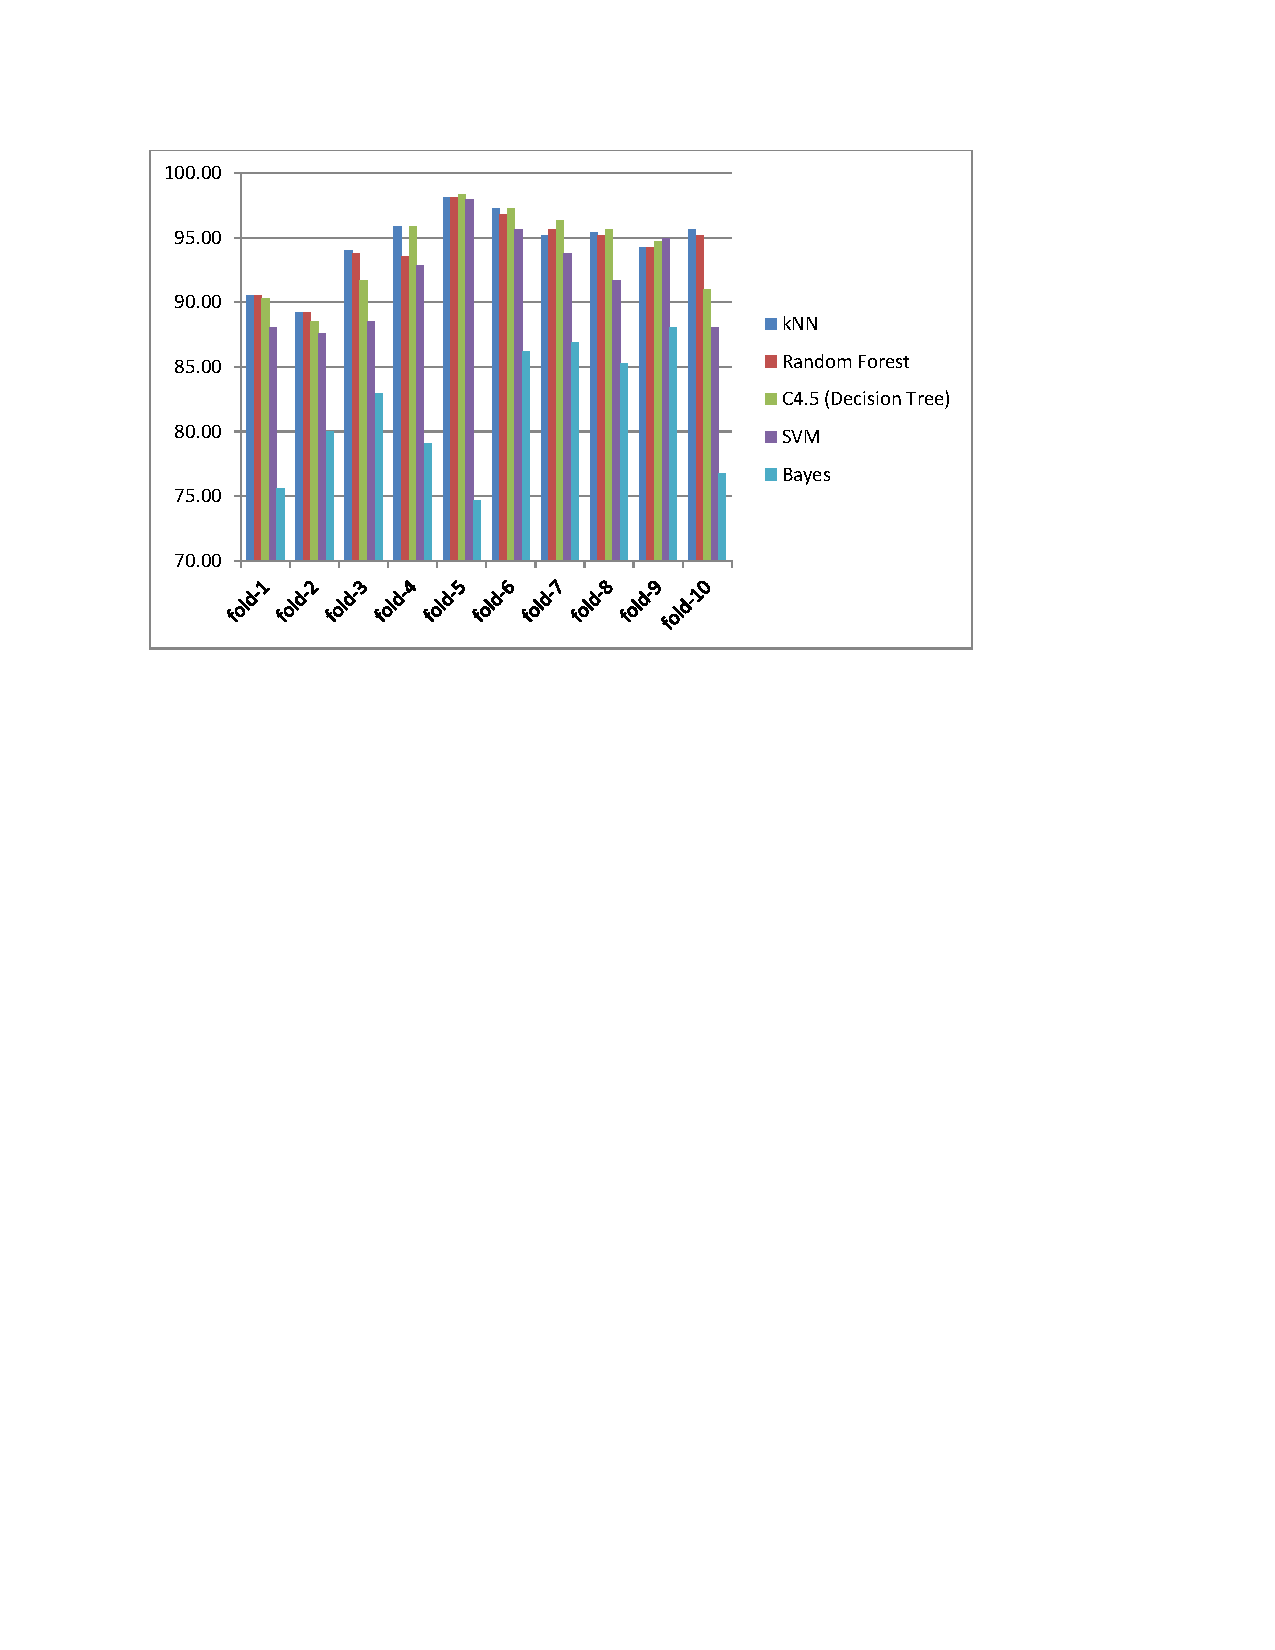
\includegraphics[width=0.9\textwidth]{Figure_A_5.pdf}
%  \caption{Trực quan độ chính xác giải quyết nhập nhằng với đánh giá chéo 10-fold trên tập đặc trưng đề xuất và các bộ phân lớp khác nhau}\label{fig:figure_A_5}
%\end{center}  
%\end{figure}